\section{The Competitive Landscape: Why No Existing Platform Fills the Gap}
\label{sec:landscape}

Sections~\ref{sec:history}--\ref{sec:solution} compared TrustBazaar with Bikroy. Bikroy is not the only
option, however: Facebook and Daraz also carry resale and online sales. This section compares
TrustBazaar with every realistic alternative available to a Bangladeshi reselling a used item
today, including digital items such as game accounts and event tickets, and shows that the
combination TrustBazaar offers does not exist in the market.

\subsection{Bikroy under Jiji}

Since May 2026 Bikroy runs on Jiji's platform~\cite{fs_jiji}. Jiji's safety model is the same
as Bikroy's: it moderates ads before publication, uses automated fraud detection, and instructs
buyers never to pay before receiving an item, but it does not hold the payment
itself~\cite{jiji_kenya}. The acquisition gave Bikroy a new owner, not a new trust model.

\subsection{Facebook Marketplace and buy-and-sell groups}
\label{sec:facebook}

Facebook Marketplace has launched in Bangladesh, but Facebook does not facilitate payment or
delivery for person-to-person Marketplace sales, and as of 2021 its Shops checkout was not
available in Bangladesh~\cite{fs_facebook}. Buyers and sellers therefore settle outside the
platform, exactly as on Bikroy.

Scams on Facebook follow the same advance-payment pattern documented in
Section~\ref{sec:users}. In February 2021, Dhaka police arrested five members of a gang that
advertised goods on a Facebook page, took 50\% advance payments plus delivery charges, and then
shut down both the page and the mobile-banking account. The gang had been operating for about
six months and had opened its accounts using \emph{fake national identity documents}, which
made it hard to trace~\cite{tbs_fcommerce}. This last detail matters for TrustBazaar and is
discussed in Section~\ref{sec:threats}.

\subsubsection*{Digital goods: game accounts, tickets and the ``admin deal''}

Facebook buy-and-sell groups are also used to trade \emph{digital} goods: accounts for games
such as PUBG Mobile, Free Fire and Clash of Clans, Steam or Epic Games accounts, and event
tickets. These items cannot be inspected like a phone. In the groups our team is familiar with,
the usual way to manage the risk is an ``admin deal'', in which the group's admin acts as a
middleman: the buyer sends the money to the admin, the seller
sends the account ID and password to the admin, and the admin passes each on
(Figure~\ref{fig:admin_deal}). We did not find a published study measuring how often these
deals fail, but the available evidence shows why the structure itself is unsafe.

\begin{figure}[H]
  \centering
  \resizebox{0.97\textwidth}{!}{% The Facebook-group "admin deal" for digital goods, and its failure modes
\begin{tikzpicture}[
  font=\footnotesize,
  party/.style={draw=#1, fill=#1!12, rounded corners=3pt, minimum width=2.6cm,
                minimum height=1.0cm, align=center, font=\footnotesize\bfseries},
  tr/.style={-{Stealth[length=2mm]}, thick, draw=#1},
  lab/.style={font=\scriptsize, fill=white, inner sep=1.5pt, align=center},
  fail/.style={draw=bad, fill=bad!7, rounded corners=2pt, text width=4.1cm,
               align=left, font=\scriptsize, inner sep=4pt}]

  \node[party=good]  (B) at (0,0)    {Buyer};
  \node[party=muted] (A) at (6,0)    {Group admin\\{\scriptsize\normalfont (unverified, unaccountable)}};
  \node[party=good]  (S) at (12,0)   {Seller};

  \draw[tr=good] ([yshift=3mm]B.east) -- node[lab, above]{1. money} ([yshift=3mm]A.west);
  \draw[tr=good] ([yshift=3mm]S.west) -- node[lab, above]{2. ID + password} ([yshift=3mm]A.east);
  \draw[tr=ink]  ([yshift=-3mm]A.west) -- node[lab, below]{3. credentials} ([yshift=-3mm]B.east);
  \draw[tr=ink]  ([yshift=-3mm]A.east) -- node[lab, below]{4. money} ([yshift=-3mm]S.west);

  \node[fail] (f1) at (0,-2.6)
    {\textbf{Admin + seller collude:} buyer's money kept, or the account is handed over
     and later recovered by the seller.};
  \node[fail] (f2) at (6,-2.6)
    {\textbf{Admin acts alone:} holds both the money and the credentials with no identity
     on record and nobody to answer to.};
  \node[fail] (f3) at (12,-2.6)
    {\textbf{Admin + buyer collude:} seller hands over the account and is never paid.};

  \draw[-{Stealth[length=1.6mm]}, bad, densely dashed] (f1.north) -- (B.south);
  \draw[-{Stealth[length=1.6mm]}, bad, densely dashed] (f2.north) -- (A.south);
  \draw[-{Stealth[length=1.6mm]}, bad, densely dashed] (f3.north) -- (S.south);
\end{tikzpicture}
}
  \caption{The Facebook-group ``admin deal'' for digital goods. A single unverified person holds
  both the money and the credentials, which allows three kinds of fraud. Risks of account
  transfer as described by Supercell~\cite{supercell_fairplay}; admin misconduct illustrated by
  the 2026 BCEC case~\cite{fe_bcec}.}
  \label{fig:admin_deal}
\end{figure}

\begin{itemize}
  \item \textbf{Admins hold power without accountability.} In July 2026 the Criminal
  Investigation Department (CID) arrested the 21-year-old admin of the Facebook group
  ``Bangladesh Concert \& Event Connects''. He had approved posts selling tickets for an
  Atif Aslam concert that used images of tickets from a previously cancelled concert, and when
  the organisers asked him to remove them, he demanded Tk~1~lakh instead. A case was filed under
  the Cyber Security Act at Paltan Police Station~\cite{fe_bcec}. The person members trusted to
  keep the group safe was the one exploiting it.

  \item \textbf{The game companies themselves name the risks.} Supercell's policy lists the
  dangers of buying an account: the seller may never deliver it, the same account may be sold
  to several buyers, and the original owner may keep access and take it back. Supercell also
  permanently bans accounts confirmed to have changed hands~\cite{supercell_fairplay}.

  \item \textbf{Account sales break the publishers' terms.} Steam's Subscriber Agreement forbids
  sharing a password or letting others use an account, and does not allow accounts to be sold or
  transferred (Section~1.C)~\cite{steam_ssa}. Garena's terms for Free Fire make accounts
  non-transferable and for personal use only (Section~6.2)~\cite{sk_garena}. A buyer can
  therefore lose a purchased account to a ban even if the seller is honest.

  \item \textbf{The same fraud appears in the region.} In September 2022 Pakistan's Federal
  Investigation Agency arrested suspects in Faisalabad for selling fake PUBG accounts; one
  complainant alone had lost about PKR~820{,}000~\cite{techjuice_pubg}.

  \item \textbf{Bikroy offers no answer either.} Bikroy hosts game-account listings, for example
  a Free Fire account advertised for BDT~9{,}500 in 2020, but shows the same safety tips it uses for
  physical goods: meet in a safe public place and inspect the item before
  paying~\cite{bikroy_ff}. That advice cannot be followed for a password.

  \item \textbf{Large platforms have recognised the problem.} In July 2025 Steam introduced a
  seven-day trade-protection window during which item trades can be reversed, specifically to
  counter scams and compromised accounts~\cite{pcworld_steam}. The industry's own answer to
  digital-goods fraud is a holding period, the same principle as escrow.
\end{itemize}

Digital goods therefore combine every weakness identified in this report. There is nothing to
inspect, identities are unverified, the money moves first, and the only safeguard is a single
unaccountable middleman. The revised TrustBazaar proposal therefore adds a dedicated
game-account escrow, in which ownership is verified before listing, credentials are encrypted
so that only the buyer can read them, and payment is held through a protection period after
takeover~\cite{proposal_rev}. Because account trading conflicts with the publishers' terms, the
proposal discloses that risk to buyers before payment rather than presenting these sales as
approved by the publisher.

\subsection{Daraz}

Daraz does protect buyers. Since October 2025 it has offered a 14-day return window on
applicable items, with free pickup or drop-off and refunds that include delivery
charges~\cite{pa_daraz}. However, Daraz is built for businesses selling new stock: according to
our proposal's market review, its seller requirements are built around business registration
rather than personal identity checks, and it offers no auction format~\cite{proposal}. It is not
designed for one person selling one used item to another.

\subsection{Side-by-side comparison}

Table~\ref{tab:landscape} and Figure~\ref{fig:capabilities} compare the four platforms on the
capabilities this report has shown to matter.

\begin{table}[H]
  \centering
  \small
  \caption{Capabilities of the main platforms available for resale in Bangladesh.}
  \label{tab:landscape}
  \begin{tabularx}{\textwidth}{@{}>{\raggedright\arraybackslash}p{2.6cm}
     >{\raggedright\arraybackslash}X >{\raggedright\arraybackslash}X
     >{\raggedright\arraybackslash}X >{\raggedright\arraybackslash}X@{}}
    \toprule
    \textbf{Capability} & \textbf{Bikroy / Jiji} & \textbf{Facebook} & \textbf{Daraz} &
      \textbf{TrustBazaar} \\
    \midrule
    Built for individuals' used goods & Yes & Yes & No: businesses, new stock~\cite{proposal}
      & Yes \\
    Identity verification & Phone OTP~\cite{fs_fraud} & Facebook account only;
      fake NIDs used~\cite{tbs_fcommerce} & Business registration~\cite{proposal}
      & NID + selfie KYC \\
    Who holds the payment & Nobody~\cite{bikroy_terms,jiji_kenya} & Nobody~\cite{fs_facebook}
      & Platform checkout & Escrow until receipt \\
    Refund if item is bad or missing & No; liability $\le$ BDT~6{,}700~\cite{bikroy_terms}
      & No & Yes, 14-day returns~\cite{pa_daraz} & Yes, dispute while funds are held \\
    Handover & Meet in person~\cite{bikroy_safety} & Arranged by users
      & Platform logistics~\cite{pa_daraz} & Safe meetup point or booked courier \\
    Dispute process & None~\cite{bikroy_terms} & Group admin at best~\cite{fe_bcec}
      & Returns process & Operator decision using ledger \\
    Fair auction & No & Informal comment bidding~\cite{proposal} & No~\cite{proposal}
      & Server-timed, anti-sniping \\
    Digital goods & Listed with physical-goods advice~\cite{bikroy_ff} & Admin deals
      & Not examined & Game-account escrow~\cite{proposal_rev} \\
    \bottomrule
  \end{tabularx}
\end{table}

\begin{figure}[H]
  \centering
  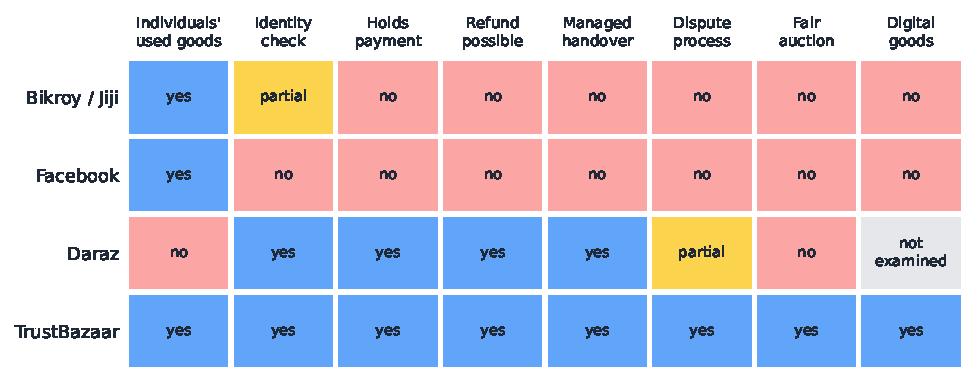
\includegraphics[width=\textwidth]{fig16_capabilities.pdf}
  \caption{Capability matrix of Table~\ref{tab:landscape}. Blue: yes; yellow: partial; red: no;
  grey: not examined. Daraz's identity and auction entries come from
  our proposal's market review~\cite{proposal}; all other sources are given in
  Table~\ref{tab:landscape}.}
  \label{fig:capabilities}
\end{figure}

\subsection{The empty quadrant}

Two questions separate the platforms: \emph{who is it built for} (individuals selling used goods,
or businesses selling new stock), and \emph{does the platform protect the transaction} (hold the
money, offer refunds, resolve disputes)? Bikroy and Facebook are built for individuals but
protect nothing. Daraz protects the transaction but is built for businesses. No existing
platform does both (Figure~\ref{fig:positioning}).

\begin{figure}[H]
  \centering
  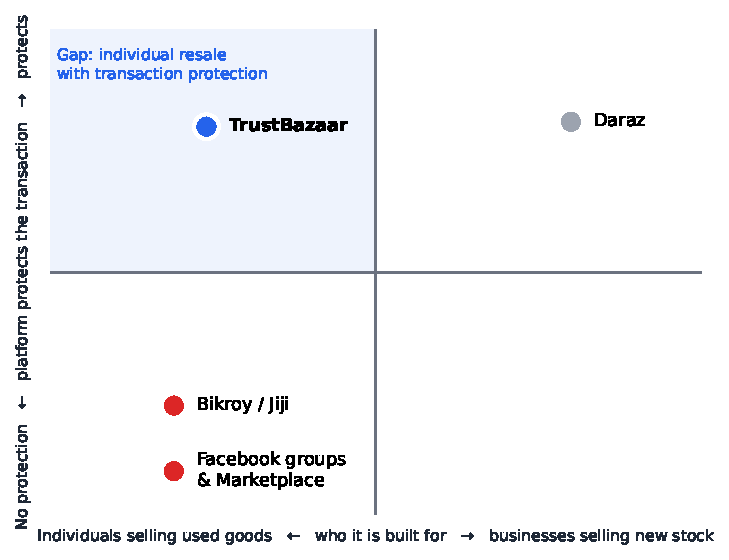
\includegraphics[width=0.72\textwidth]{fig17_positioning.pdf}
  \caption{Qualitative positioning of the platforms, based on the capabilities in
  Table~\ref{tab:landscape}. Positions show which quadrant each platform belongs to, not a
  measured score.}
  \label{fig:positioning}
\end{figure}

Each existing platform proves half of TrustBazaar's case. Bikroy and Facebook prove the
\emph{demand}: hundreds of thousands of individuals resell used goods online every
month~\cite{fs_jiji}. Daraz and the 2021 escrow rule prove that the \emph{protection} works and
that Bangladeshi buyers accept platform-managed payments and returns~\cite{pa_daraz,tbs_escrow}.
TrustBazaar combines the two.

\subsection{Threats and honest limits}
\label{sec:threats}

\begin{table}[H]
  \centering
  \small
  \caption{Competitive threats and our assessment.}
  \label{tab:threats}
  \begin{tabularx}{\textwidth}{@{}>{\raggedright\arraybackslash}p{3.6cm} Y@{}}
    \toprule
    \textbf{Threat} & \textbf{Assessment} \\
    \midrule
    Fake NIDs can defeat KYC, as the 2021 Facebook gang showed~\cite{tbs_fcommerce}
      & KYC raises the cost of fraud; it does not eliminate it. TrustBazaar adds a selfie match and
        operator review~\cite{proposal}. More importantly, escrow means a fake identity still
        cannot take the buyer's money: payment is released only when the buyer confirms
        receipt. Identity checks and escrow cover each other's gaps. \\
    \addlinespace
    Daraz could open to individuals' used goods
      & Possible. If it did, that would confirm the gap is real; TrustBazaar's auction and
        person-to-person delivery design would still differ from Daraz's business model. \\
    \addlinespace
    Jiji could add escrow to Bikroy
      & Also possible. So far Jiji's stated model is pay-on-delivery advice, not held
        payments~\cite{jiji_kenya}. \\
    \addlinespace
    Facebook's reach
      & Facebook's user base cannot be matched. TrustBazaar's case is not reach but the one thing
        Facebook does not offer for person-to-person deals in Bangladesh: holding the
        money~\cite{fs_facebook}. \\
    \bottomrule
  \end{tabularx}
\end{table}

TrustBazaar's advantage is its design, not a barrier competitors cannot copy. The project's aim is to
show that this design can be built correctly,
with concurrency-safe auctions and escrow that never releases money wrongly~\cite{proposal},
not to claim that incumbents can never follow.

\subsection{Summary}

Every platform available to a Bangladeshi reseller today fails on at least one of two counts.
Bikroy, Jiji and Facebook serve individuals but leave the transaction to chance, and for digital
goods they leave it to an unaccountable group admin. Daraz protects the transaction but is not
built for individuals reselling used goods. TrustBazaar is designed to combine both. Its case for adoption
rests not on the other platforms being poor at what they do, but on none of them doing this.
